\section{Theorie}
\label{sec:Theorie}

\subsection{Grundlagen}
\label{sec:grundlagen}

\subsection{Reflexion}
\label{sec:reflexion}
\begin{figure}[H]
    \centering
    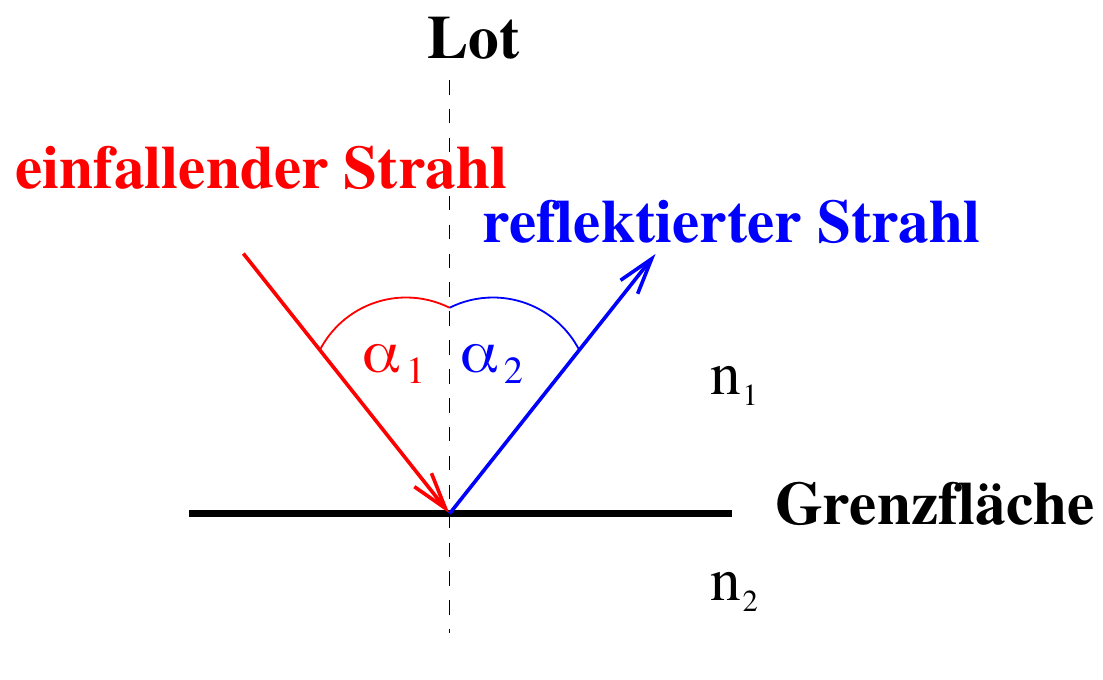
\includegraphics[scale = 0.3]{pictures/Reflexion.png}
    \caption{Reflexion eines Lichtstrahls. Quelle: \cite{AP01}}
    \label{fig:reflexion}
\end{figure}

\subsection{Brechung}
\label{sec:brechung}
\begin{figure}[H]
    \centering
    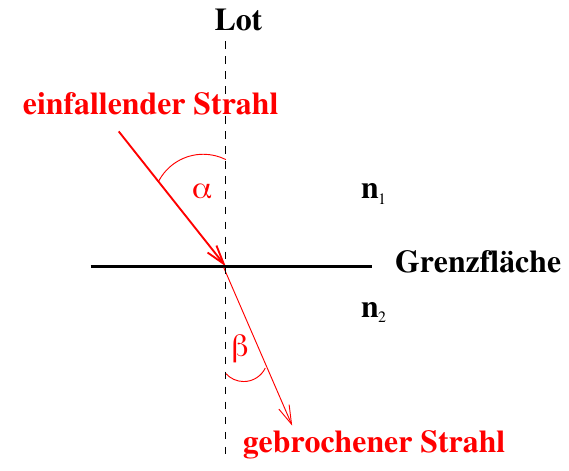
\includegraphics[scale = 0.5]{pictures/Brechung.png}
    \caption{Brechung eines Lichtstrahls. Quelle: \cite{AP01}}
    \label{fig:brechung}
\end{figure}

\subsection{Reflexion und Transmission}
\label{sec:RefTrans}
\begin{figure}[H]
    \centering
    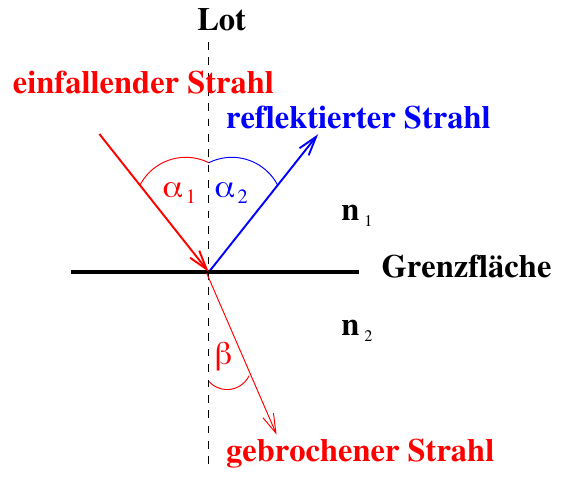
\includegraphics[scale = 0.5]{pictures/ReflexionTransmission.png}
    \caption{Reflexion und Transmission eines Lichtstrahls. Quelle: \cite{AP01}}
    \label{fig:reflexion}
\end{figure}

\subsection{Beugung}
\label{sec:beugung}